\documentclass[12pt]{article}
\usepackage[margin=0.7in]{geometry} 		% defines page margin
\usepackage{knitting} 				% defines \chart and \textknit
\usepackage{titling} 				% title page
\usepackage{graphicx,xspace, scrextend}	% defines space control stuff
\usepackage{tabularx, array, colortbl}	% defines tables
\usepackage{multicol} 				% defines columns
\usepackage{multirow} 				% defines multirows, combined cells in tables
\usepackage{framed} 				% defines boxes for notes and written directions
\usepackage{xstring}				% StrSubstitute
\usepackage[x11names]{xcolor} 		% extends color library
\usepackage{hyperref}				% hyperlinks
\hypersetup{
    colorlinks=true,
    linkcolor=blue,
    filecolor=magenta,      
    urlcolor=blue,
}
\pdfmapfile{+knitfont.map}

% font selection
\usepackage{palatino, moresize, sectsty}
\allsectionsfont{\sffamily}

\renewcommand{\arraystretch}{2} % compresses tables for pattern keys

\newcolumntype{L}[1]{>{\leftalign\arraybackslash}p{#1}}
\newcolumntype{C}[1]{>{\centering\arraybackslash}p{#1}}

% length parameters
\setlength{\parindent}{0pt} % disables indentation for paragraphs
\setlength{\columnsep}{0.7cm} % column separation in multicol environment

% color parameters
\colorlet{framecolor}{black}
\colorlet{shadecolor}{LemonChiffon1}
\colorlet{highlight}{yellow}

% COLORWORK?!
\colorlet{MC}{purple!50}
\colorlet{CCA}{green}
\colorlet{CCB}{white}

\newcommand{\makeActive}{
	\catcode`\0=\active % MC
	\catcode`\1=\active % CC1
	\catcode`\2=\active % CC2
}	% define additional colors as needed

% plain knit colorwork symbols are defined with charts
% how to get other symbols (increases/decreases)
\newcommand{\MC}[1]{\purlpass{\color{MC}}\purlbackground{#1}}
\newcommand{\CCA}[1]{\mainpass{\color{black}}\purlpass{\color{CCA}}\purlbackground{#1}}
\newcommand{\CCB}[1]{\mainpass{\color{black}}\purlpass{\color{CCB}}\purlbackground{#1}}

% custom commands
\newcommand{\comment}[1]{} % allows for multiline comments that LaTeX will ignore

\newcommand{\vocab}[1]{\emph{\textbf{#1}}} % format for highlighting definitions of stitches, vocabulary terms
\newcommand{\rowDir}[1]{\textbf{#1:}} % indent for written instructions within paragraphs

\renewcommand{\repeat}[1]{\textbf{\textasteriskcentered[#1]}, repeat from \textasteriskcentered \hspace{1pt}} % format for written repeats, bold with *[ stitches ]*
\newcommand{\x}{$\times$}			% times symbol but shorthand
\newcommand{\setrepeat}[2]{\textbf{[#1]}\x{#2}}		% format for repeats with set number of repetitions, bold with [ stitches ]

\newcommand{\blank}{\underline{\hspace{2em}} } % written instructions, fill-in-the-blank box
\newcommand{\highlighted}[1]{\colorbox{highlight}{#1}} % written instructions, highlight particular text


% stitch count commands
\newcommand{\increase}[1]{(\emph{+#1 
	\ifnum#1=1{st}\else{sts}\fi})}
\newcommand{\decrease}[1]{(\emph{$-$#1
	\ifnum#1=1{st}\else{sts}\fi})}
\newcommand{\stitchcount}[1]{(\emph{#1 sts})}

% marker instructions
\renewcommand{\pm}[1]{\emph{pm #1}} % place stitch marker
\newcommand{\sm}{\emph{sm}} % slip marker
\renewcommand{\rm}[1]{\emph{rm #1}} % remove stitch marker

% thick horizontal line
\makeatletter \newcommand{\thickhline}{
    \noalign {\ifnum 0=`}\fi \hrule height 1.5pt
    \futurelet \reserved@a \@xhline
}
\makeatother

% custom environments
\newenvironment{frnote}
    {% framed environment for pattern notes
    	\setlength{\FrameRule}{1.5pt}
    	\def\FrameCommand{\fboxrule=\FrameRule\fboxsep=\FrameSep \fcolorbox{framecolor}{shadecolor}}
    	\MakeFramed {\FrameRestore}}
    {\setlength{\FrameRule}{1pt}
	\endMakeFramed}

\newenvironment{frdirection}
    {% framed environment for written directions
	\def\FrameCommand{\fboxrule=\FrameRule\fboxsep=\FrameSep \fbox}
   	\MakeFramed {\advance\hsize-\width \FrameRestore}
    	\addmargin[1.5cm]{0pt}}
    {\endaddmargin
	\endMakeFramed}

\newenvironment{unframed}
    {% unframed environment for written directions
	\begin{addmargin}[2em]{0pt}
	\setlength{\parindent}{-2em}}
    {%\vspace{1em}
	\setlength{\parindent}{0em}
	\end{addmargin}}

\title{Druid Circle Sweater} % pattern name here
\author{Shanel Wu (Piper Nell)}

\begin{document}

%%%%%%%%%%%%%%%%%%%%%%%%%%%%%%%%%%%%%%%%%%%%%%%%%%
% TITLE PAGE 

% COVER PHOTO
\begin{center}
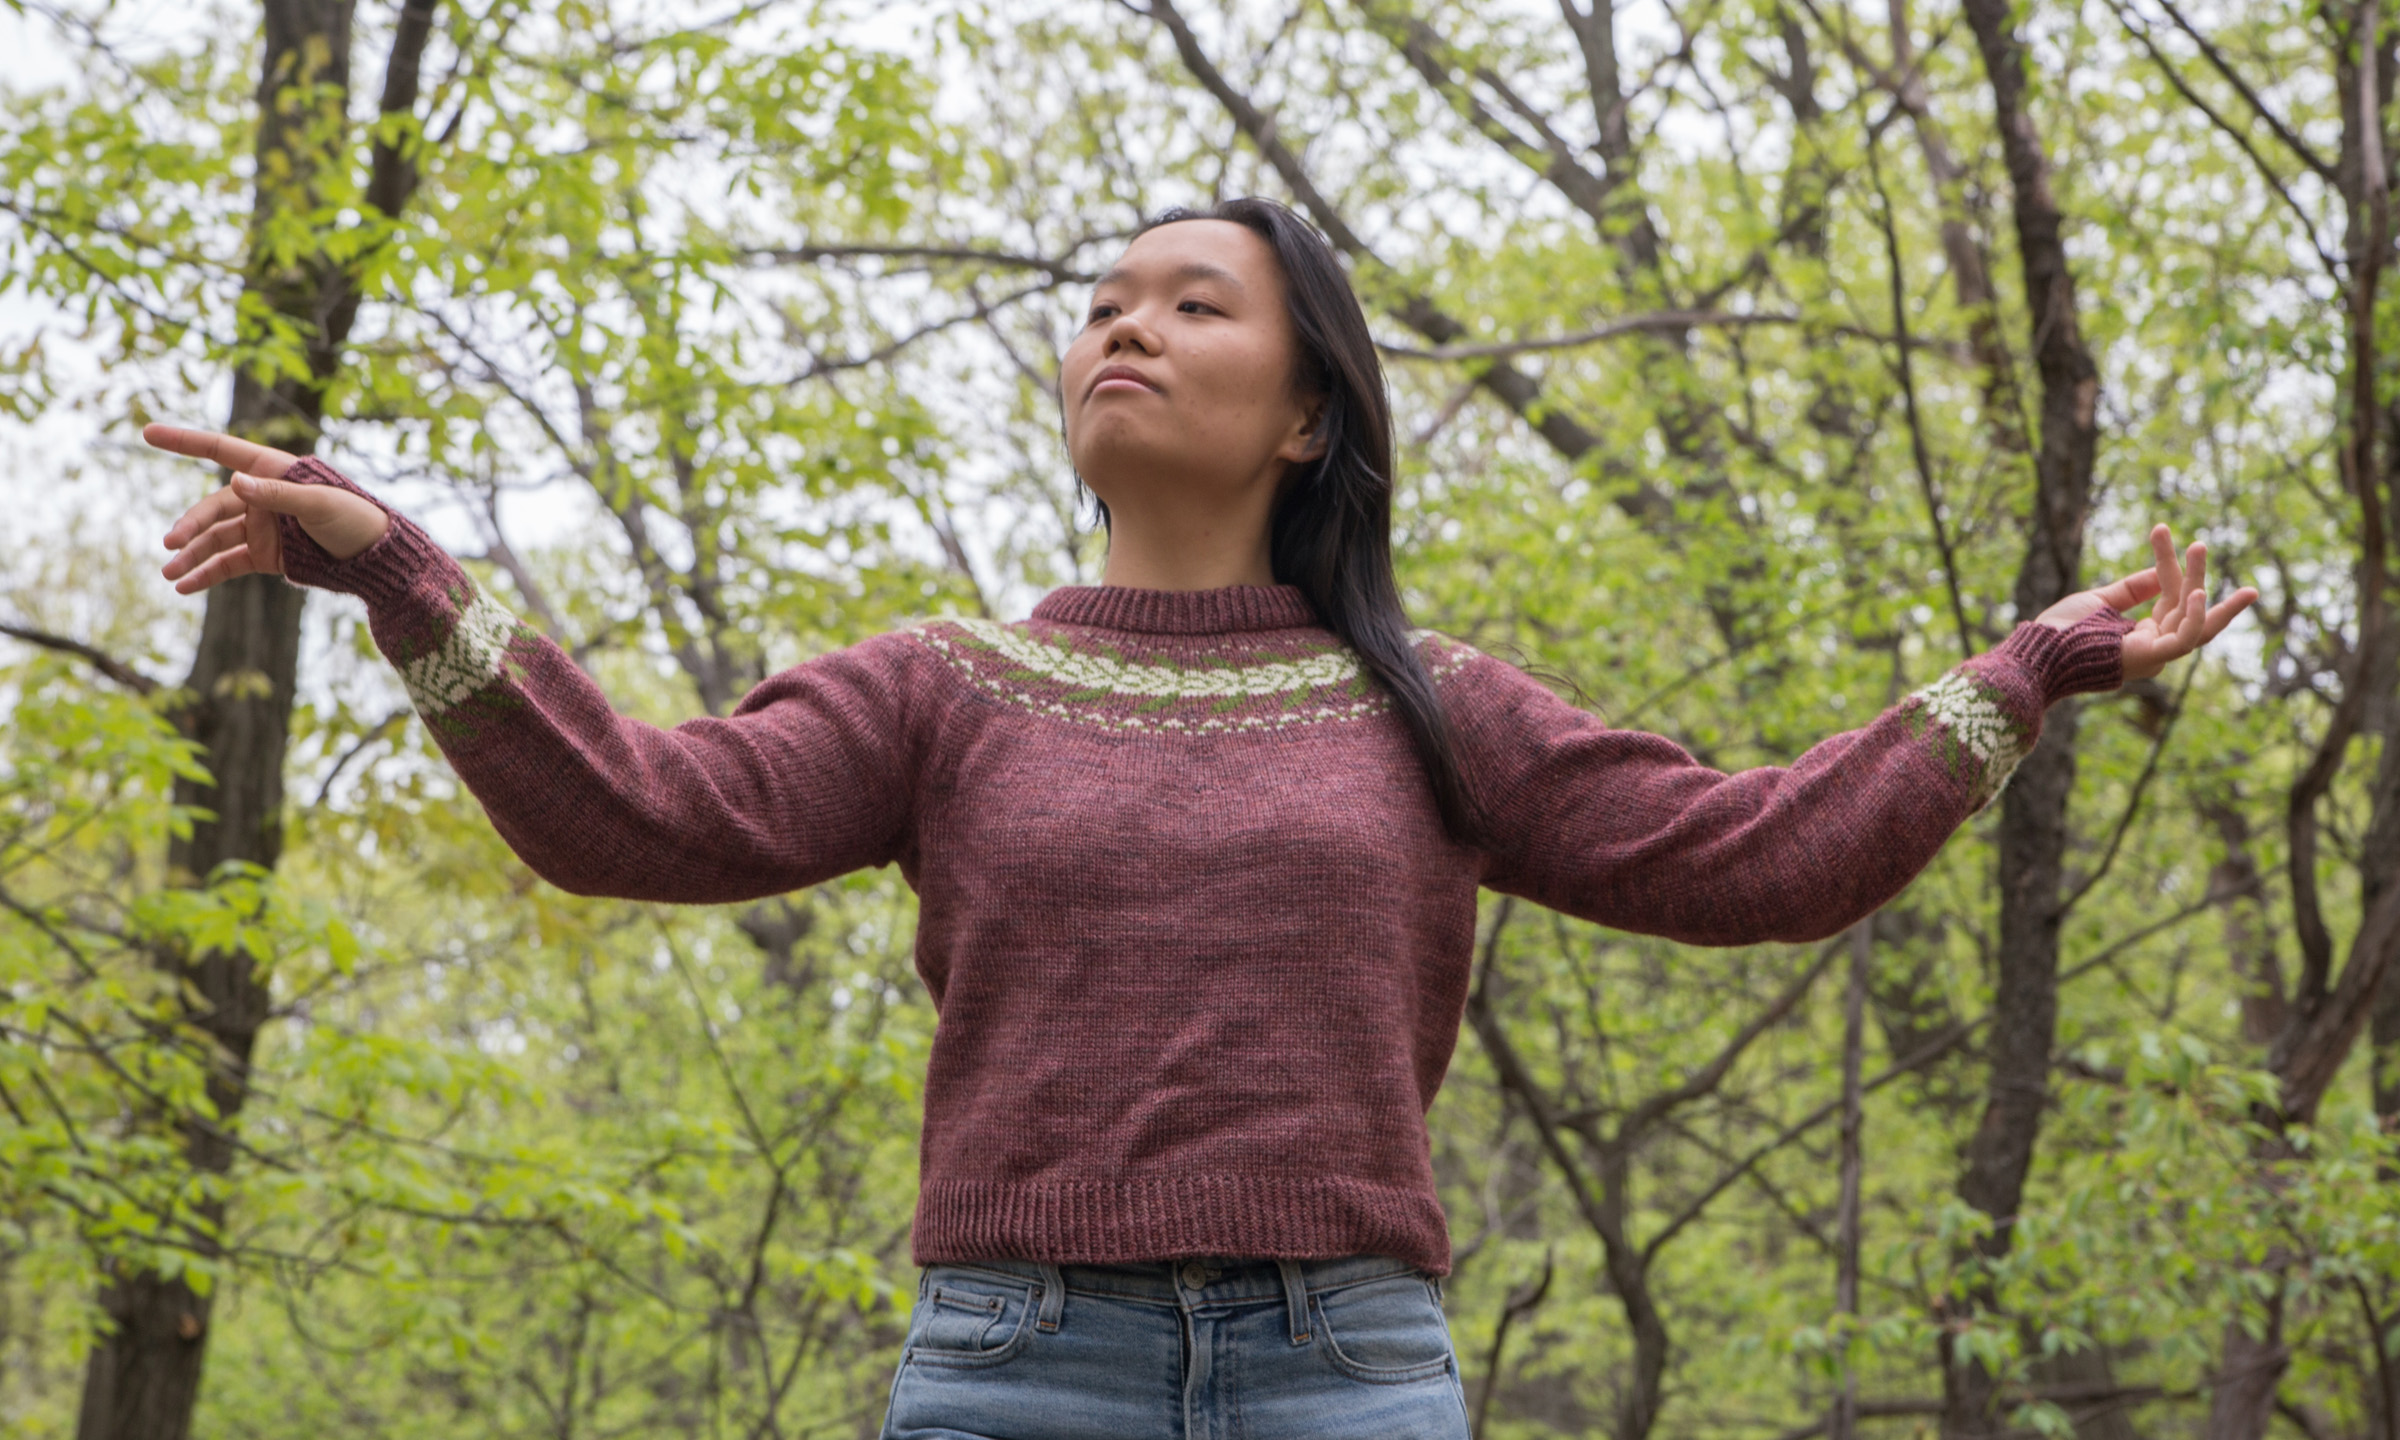
\includegraphics[width=7in]{pointing.jpg}
\end{center}

% uncommend line below if you want a background fill image
% \ThisLRCornerWallPaper{1.0}{image.jpg} 

{\fontfamily{qag}\selectfont
\HUGE\textbf{\thetitle}
\hspace{0.5em} % adjust this space
\normalsize\theauthor
}

\begin{multicols}{2}

% Cute description here
In fantasy settings, I am often drawn towards the primal magics of druids. The leaf-inspired colorwork on this top-down, circular-yoke sweater evokes the druid's connection to their land. With customizable shaping, thumb holes, and a folded collar, this sweater will be excellent for morning hikes.

\subsection*{Sizing}

This pattern is written in gender-neutral sizes XS (S, M, L) (XL, 2L, 3L) corresponding to a finished chest dimension of 
32 (36, 40, 44) (48, 52, 56)" or 
80 (90, 100, 110) (120, 130, 140) cm, 
with an intended positive ease of 2-4" or 5-10cm in the chest. See schematic on next page for complete dimensions and sizing details.

\subsection*{Gauge}

6 sts x 8 rows = 1"/2.5cm or 24 sts x 32 rows = 4"/10cm in stockinette with size A needles and MC, after gentle blocking.

% sample measurements, gauge, notes on ease, etc.

\subsection*{Yarn Requirements}

% yardage, number of colors, etc.
Sport or DK weight yarn in a main color (MC) and two contrasting colors (CC1 and CC2)

 \textbf{MC:} 700 (850, 1050, 1300) (1500, 1800, 2000) yds

\textbf{CC1:} 90 (90, 90, 90) (100, 105, 105) yds

\textbf{CC2:} 80 (80, 80, 85) (90, 95, 95) yds

% also include: sample yarn, other yarn suggestions

\subsection*{Needles}

\textbf{Size A (for main fabric)}
\begin{itemize}
\item 16" circular needle in size needed to obtain gauge. \emph{Suggested: US 4/3.5mm}
\item 32" circular needle in the same size.
\end{itemize}

\textbf{Size B (for ribbing)}
\begin{itemize}
\item 32" circular needle one size smaller than Size A.
\item \emph{(optional)} 16" circular needle or DPN's for sleeve cuffs and collar.
\end{itemize}
\vfill

\newpage
\subsection*{Other Tools \& Notions}

Stitch markers, waste yarn, tapestry needle.

\subsection*{Techniques}

This pattern is suitable for an advanced beginner with some familiarity with stranded colorwork and top-down sweater construction.
Prior to knitting this pattern, you should be comfortable with knitting in the round, increasing \& decreasing, and simple stranded colorwork. Colorwork is charted only, with no floats longer than 5 stitches. 

Some support is provided for wrap \& turn short row shaping, the tubular bind off, and modifying to fit your body.
Pattern Key describes all abbreviations and describes stitches used.


%%%%%%%%%%%%%%%%%%%%%%%%%%%%%%%%%%%%%%%%%%%%%%%%%%
% FOREWORD

\subsection*{Notes on Fit}

The Druid Circle sweater is designed to be worn with positive ease in the chest and arms. To determine your chest measurement, measure the widest part of your chest. To determine your upper arm measurement, measure the widest part of your upper arm. Choose the size with a chest circumference that is 2-4" or 5-10 cm larger than your chest measurement. Body and sleeve lengths can be adjusted as outlined in the \textbf{Modification Suggestions}.

% Sizing/Schematic/Notes on Fit
\section*{Schematic}
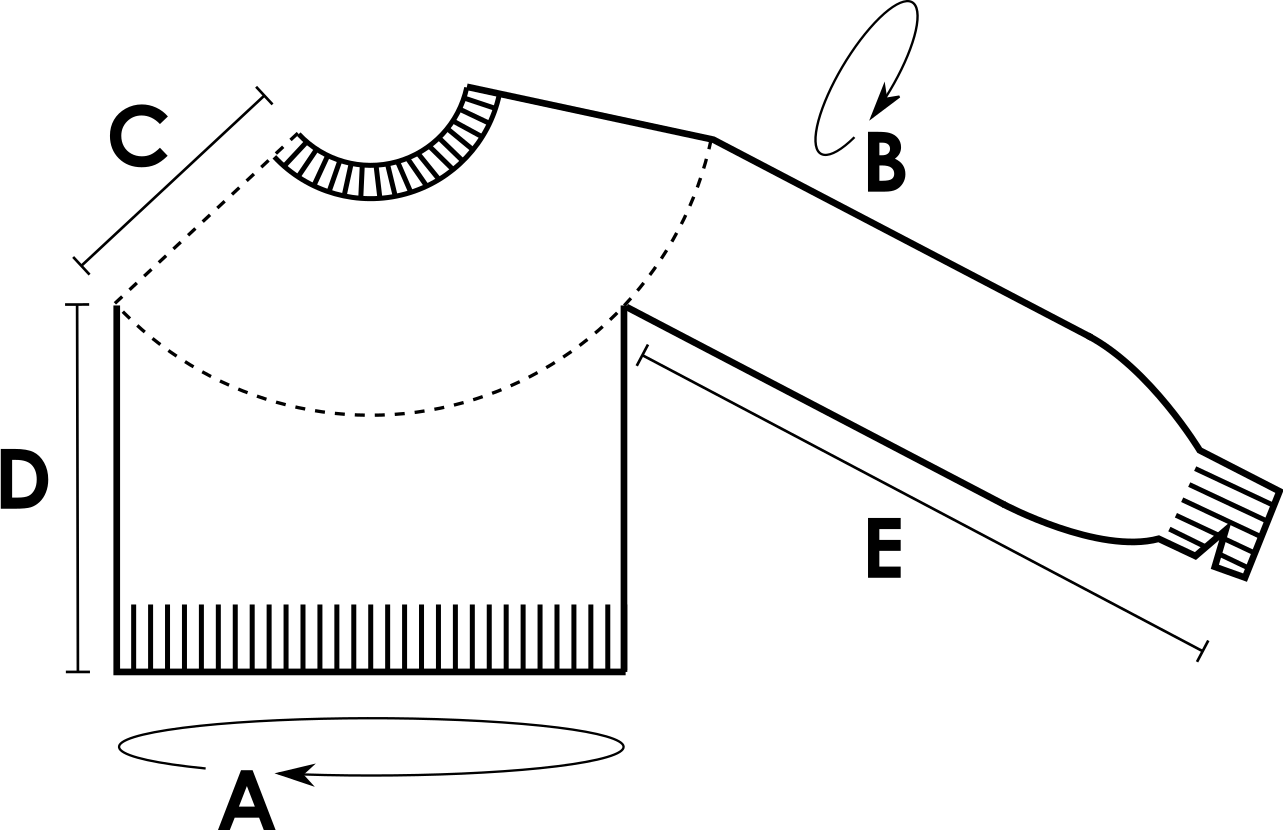
\includegraphics[width=4in]{schematic.png}



% Measuring yourself to fit
\columnbreak

\subsection*{Pattern Key}

% formatting notes for charts and written directions

\vocab{Written instructions:} 

repeats = \repeat{stitches} to \blank

\vspace{-1em}
% stitch key - fill in with all stitches used in design: chart symbol, written abbreviation, full stitch name or explanation
% stitches with explanations must first be BOLDED, followed by colon then explanation
% discuss any special techniques and tutorials included
\begin{center}
{\renewcommand{\arraystretch}{1.2}
\begin{tabular}{| C{0.2\linewidth}  p{0.8\linewidth} | }
\thickhline \rowcolor{shadecolor} 
\textbf{Abbr.}	& \textbf{Description} \\ \thickhline
CO	& cast on \\
BO 	& bind off \\
BOR 	& beginning of round \\
MC 	& main color \\
CC1 	& contrast color 1 \\
CC2 	& contrast color 2 \\
pm	& place stitch marker \\
sm	& slip stitch marker \\
rm 	& remove stitch marker \\
k	&  knit \\
p	& purl   \\
k tbl	& knit through the back loop \\
k2tog 	& knit 2 together \\
ssk	& slip slip knit \\
m1	& \textbf{make one:} with L needle, pick up bar between sts front to back, k tbl \\
w\&t 	& \textbf{wrap \& turn:} \emph{See \textbf{Special Techniques}.} \\
st st 	& \textbf{stockinette stitch:} (worked in the round) k all sts \\
1x1 twisted ribbing 	& \repeat{k tbl, p1} to end of round \\
\hline
\end{tabular}
}
\end{center}
{\begin{addmargin}[4em]{-2em} \small
{\normalsize\textbf{\textsf{A: Chest Circumference}}} 

\hspace{1em} 32 (36, 40, 44) (48, 52, 56)"

\hspace{1em} 80 (90, 100, 110) (120, 130, 140) cm 

{\normalsize\textbf{\textsf{B: Upper Arm Circumference}}}

\hspace{1em} 13 (13.5, 14, 15) (16.5, 18.5, 20)"

\hspace{1em} 32.5 (33.75, 35, 37.5) (41.25, 46.25, 50) cm 

{\normalsize\textbf{\textsf{C: Yoke Depth}}}

\hspace{1em} 9.5 (10, 10.5, 11) (12, 13.5, 15)"

\hspace{1em} 23.75 (25, 26.25, 27.5) (30, 33.75, 37.5) cm

{\normalsize\textbf{\textsf{D: Body Length}}}

\hspace{1em} 10 (11, 12, 13.5) (14.5, 16, 17)"

\hspace{1em} 24.5 (27.5, 30.5, 33.5) (36.5, 39, 43) cm 

{\normalsize\textbf{\textsf{E: Sleeve Length}}}

\hspace{1em} 18.5 (19, 19.5, 20) (20.5, 21, 21.5)"

\hspace{1em} 46.25 (47.5, 48.75, 50) (51.25, 52.5, 53.75) cm
\end{addmargin}}
\end{multicols}

\newpage
\begin{multicols}{2}

%%%%%%%%%%%%%%%%%%%%%%%%%%%%%%%%%%%%%%%%%%%%%%%%%%
% BEGIN INSTRUCTIONS
\section*{Yoke}

With larger needles, using MC and the long-tail cast on, cast on 
120 (126, 126, 126) (132, 132, 132) sts. 
Pm for BOR and join in the round. Your tail marks the center of the back neckline.

\subsection*{Back Neck Shaping}

\emph{See \textbf{Special Techniques} for w\&t short rows.}

\rowDir{Short Row 1 (RS)} K 40 (42, 42, 42) (44, 44, 44) sts, 
w\&t. 

\rowDir{Short Row 2 (WS)} P 40 (42, 42, 42) (44, 44, 44) sts, 
sm, p 40 (42, 42, 42) (44, 44, 44), 
w\&t.

\rowDir{Short Row 3} K to 6 sts before last wrapped st, 
w\&t.

\rowDir{Short Row 4} P to 6 sts before last wrapped st, 
w\&t.

Repeat Short Rows 3 and 4 2 (2, 2, 3) (3, 4, 4) additional times until there are 
4 (4, 4, 5) (5, 6, 6) wrapped sts on each side. 

\rowDir{Next Rnd} K to marker, sm, k around and work all wrapped sts.

K 1 round.

\begin{frnote}
\vocab{All sizes except XS:}

\rowDir{Set Up Increase Round} \repeat{K - (21, 21, 21) (22, 22, 22) sts, m1} to end of round. \increase{6} 

120 (132, 132, 132) (138, 138, 138) sts total.
\end{frnote}

\begin{frnote}
\vocab{Sizes XL, 2L, and 3L only:}

K 1 round.

\rowDir{Set Up Increase Round 2} \repeat{K - ( - , - , - ) (23, 23, 23), m1} to end of round. \\ \increase{6}

120 (132, 132, 132) (144, 144, 144) sts total.
\end{frnote}

K 2 rounds, 
or work st st until piece measures 
1 (1, 1, 1.5) (1.5, 2, 2)" or 2.5 (2.5, 3.75) (3.75, 5, 5) cm long from the back neckline. Join CC1 and CC2. Work Yoke Chart rows 1-29, repeating a total of 
20 (22, 22, 22) (24, 24, 24) times around. You may wish to place a stitch marker between each repeat. As the piece grows, switch to longer circular needle when needed.

\vfill
\columnbreak

\begin{frnote}
\textbf{TIP:} When working a m1 increase in colorwork, make sure the bar you pick up is the same color as the yarn you use for the stitch.
\end{frnote}

\subsection*{Yoke Chart}

\textknit{\MC{-}} MC \hspace{2em}
\textknit{\CCA{-}} CC1 \hspace{2em}
\textknit{\CCB{-}} CC2 

\vspace{1em}
\textknit{v} m1 with indicated color

\begin{center}
{\makeActive
\gdef0{\leavevmode{\purlpass{\color{MC}}=}}
\gdef1{\leavevmode{\purlpass{\color{CCA}}=}}
\gdef2{\leavevmode{\purlpass{\color{CCB}}=}}
\chart[right]{
\mainpass{\color{black}}
\gridpass{\color{gridcolor}}
020002020002
011011011011
002220002220
200200200200
0\MC{v}00000000\MC{v}0
~0001000110
~0010011100
~0100111100
~1001111000
~0001110001
~0011100010
~2211222122
~2212221222
~1122212211
~2\CCB{v}121221\CCB{v}2
~~22122122
~~21212212
~~12221221
~~21222122
~~21122212
~~00110001
~~10111000
~~00011100
~~00001110
~~0\MC{v}0000\MC{v}0
~~~000020
~~~000202
~~~020000
~~~010000
}} \end{center}

Upon completing the Yoke Chart, you should have 240 (264, 264, 264) (288, 288, 288) sts total. 
Break CC1 and CC2, continuing in MC.

\newpage
% additional shaping
\subsection*{Additional Yoke Shaping}
K 4 rounds, then work Yoke Increase Round 1. Continue to knit 9 rounds ($\sim$1.25"/3cm), 
then work the next increase round, stopping after Yoke Increase Round 2 (2, 2, 3) (3, 4, 5). Each numbered Yoke Increase Round will add 40 (44, 44, 44) (48, 48, 48) sts to total.

\rowDir{Yoke Increase Round 1} \repeat{k1, m1, k10, m1, k1} to end of round. 

\rowDir{Yoke Increase Round 2} \repeat{k1, m1, k12, m1, k1} to end of round.

\rowDir{Yoke Increase Round 3} \repeat{k1, m1, k14, m1, k1} to end of round.

\rowDir{Yoke Increase Round 4} \repeat{k1, m1, k16, m1, k1} to end of round.

\rowDir{Yoke Increase Round 5} \repeat{k1, m1, k18, m1, k1} to end of round.

\begin{frnote}
\vocab{Sizes M, L, XL, 2L only}

K 9 rounds and then work the Final Yoke Increase Round to add - ( - , 22, 22) (24, 24, - ) sts to total.

\rowDir{Final Yoke Increase} \repeat{K - ( -, 16, 18) (18, 20, - ) sts, m1} to end of round.
\end{frnote}

After the last increase round, work st st until piece measures 
9.5 (10, 10.5, 11) (12, 13.5, 15)" or 23.75 (25, 26.25, 27.5) (30, 33.75, 37.5) cm from back neckline.

Before separating for the body and sleeves, you should have 
320 (352, 374, 418) (456, 504, 528) sts total. At this point, you may wish to look at \vocab{Modification Suggestions} for the body.

\subsection*{Separate for Body and Sleeves}

In this round, use the backwards loop cast on for underarm CO's. Sm at BOR, k 
42 (48, 53, 60) (65, 72, 76), place next 
76 (80, 80, 88) (98, 108, 112) sts on waste yarn for right sleeve, CO 
12 (12, 14, 12) (14, 12, 16) sts for right underarm, k 
84 (96, 107, 121) (130, 144, 152) sts for front, place next 
76 (80, 80, 88) (98, 108, 112) sts on waste yarn for left sleeve, CO 
12 (12, 14, 12) (14, 12, 16) sts for right underarm, k to marker. You should have 
192 (216, 242, 264) (288, 312, 336) sts on the needle for the body.

\section*{Body}

Work st st until the body measures 
10 (11, 12.5, 13.5) (14.5, 16, 18)" or 
25 (27.5, 31.25, 33.75) (36.25, 40, 45) cm from underarm CO edge.  If desired, work shaping for waist or belly. \emph{See \textbf{Modification Suggestions} for shaping guidelines.} 

Switch to smaller needles and work 1x1 twisted ribbing for 2"/5cm. BO loosely for a stretchy hem. \emph{Suggested: tubular bind off. It's worth the effort! See \textbf{Special Techniques}.}


\section*{Sleeves (make two)}

Transfer sts from waste yarn to larger needles. Join MC and knit across the 
76 (80, 80, 88) (98, 108, 112) held sts. Continuing around the sleeve, pick up and knit 
6 (6, 7, 6) (7, 6, 8) sts from CO edge, pm for BOR, then pick up and knit 
6 (6, 7, 6) (7, 6, 8) more sts from CO edge. Join in the round and knit to marker.

88 (92, 94, 100) (112, 120, 128) sts total.

\subsection*{Sleeve Shaping}

\rowDir{Next Round} K 5 (5, 6, 5) (6, 5, 7) sts, k2tog, pm, k to 
7 (7, 8, 7) (8, 7, 9) sts from BOR marker, pm, ssk, k to end \decrease{2}

\rowDir{Round 1} k all sts

\rowDir{Round 2} sm, k to 2 sts from marker, k2tog, sm, k to marker, sm, ssk, k to end \\ \decrease{2}

Repeat Rounds 1 and 2 an additional 2 (3, 3, 3) (4, 4, 5) times, removing all markers except BOR on the last repeat. \\
80 (82, 84, 90) (100, 108, 114) sts total. % Sleeve decreases

\begin{frnote}
\vocab{All sizes except XS and L}

K 7 rounds ($\sim$1"/2.5cm), then work Decrease Round as follows.

\rowDir{Decrease Round} k1, k2tog, k to 3 sts from marker, ssk, k1 \decrease{2}

Repeat Decrease Round every 8 rounds an additional - (0, 1, - ) (4, 3, 6) times. 80 (80, 80, 90) (90, 100, 100) sts total. % Sleeve decreases B
\end{frnote}

Work st st until sleeve measures 
12.5 (13, 13.5, 14) (14.5, 14.5, 15)" or
31.25 (32.5, 33.75, 35) (36.25, 36.25, 37.5) cm from underarm CO edge. 

Join CC1 and CC2. Work Rounds 1-19 of the Sleeve Cuff Chart, repeating a total of 
8 (8, 8, 9) (9, 10, 10) times around. You may wish to place a stitch marker between each repeat.

\subsection*{Sleeve Cuff Chart}

\textknit{\MC{-}} MC \hspace{2em}
\textknit{\CCA{-}} CC1 \hspace{2em}
\textknit{\CCB{-}} CC2 

\vspace{1em}
\textknit{>} k2tog with indicated color \hspace{2em}
\textknit{<} ssk
\begin{center}
{\makeActive
\gdef0{\leavevmode{\purlpass{\color{MC}}=}}
\gdef1{\leavevmode{\purlpass{\color{CCA}}=}}
\gdef2{\leavevmode{\purlpass{\color{CCB}}=}}
\chart[right]{
~00001110
~00011100
~10111000
~00110001
~21122212
~21222122
~12221221
~21212212
~2\CCB{<}1221\CCB{>}2
2212122122
1122212211
2212221222
2211222122
0011100010
0001110001
1001111000
0100111100
0010011100
0001000110
}} \end{center}

Upon completing the Sleeve Cuff Chart, you should have 
64 (64, 64, 72) (72, 80, 80) sts total. Break CC1 and CC2, continuing in MC. 

% note on swapping out cuff size for bigger/smaller hands
\begin{frnote}
\textbf{NOTE:} The cuffs are written for hand sizes ranging from 7"/17.5cm to 9"/22.5cm, measured around the broadest part of the palm. As written, the XS and S cuffs fit 7"/17.5cm hands; M, L, and XL fit 8"/20cm hands; 2L and 3L fit 9"/22.5cm hands.
\\ \emph{See \textbf{Modification Suggestions} if you need to swap out the cuff size for smaller or larger hands.}
\end{frnote}

\vfill
\columnbreak

% final sleeve shaping
\subsection*{Additional Cuff Shaping}

K 1 round.

\rowDir{Cuff Decrease Round 1} k1, \repeat{k2tog, k2} to 3 sts from end of round, k2tog, k1. 48 (48, 48, 54) (54, 60, 60) sts total.

\begin{frnote}
\vocab{Sizes XS and S only}

K 4 rounds.

\rowDir{Cuff Decrease Round 2} \repeat{k4, k2tog} to end of round. \decrease{8}

40 (40, 48, 54) (54, 60, 60) sts total.
\end{frnote}

Work st st until sleeve measures 16.5 (17, 17, 17.5) (18, 18, 18.5)" or 41.25 (42.5, 42.5, 43.75) (45, 45, 46.25) cm from underarm CO edge. 

Switch to smaller needles and work
8 (8, 10, 10) (10, 12, 12) rounds of 1x1 twisted ribbing for  
1 (1, 1.25, 1.25) (1.25, 1.5, 1.5)" or 2.5 (2.5, 3, 3) (3, 3.5, 3.5) cm of ribbing.

\subsection*{Thumb Hole}

\rowDir{Round 1} Continuing in ribbing pattern, work to 
6 (6, 7, 7) (7, 8, 8) sts from end of round. Loosely BO sts until you reach the marker, rm, then BO 
5 (5, 6, 6) (6, 7, 7) more sts.

\rowDir{Round 2} Work in ribbing pattern to the last st on the needles. CO 
11 (11, 13, 13) (13, 15, 15) sts with the backwards loop method, join back in the round.

Work 8 (8, 10, 10) (10, 12, 12) more rounds for 
1 (1, 1.25, 1.25) (1.25, 1.5, 1.5)" or 2.5 (2.5, 3, 3) (3, 3.5, 3.5) cm of ribbing. BO loosely for a stretchy edge using the same method as the body.

\begin{center}
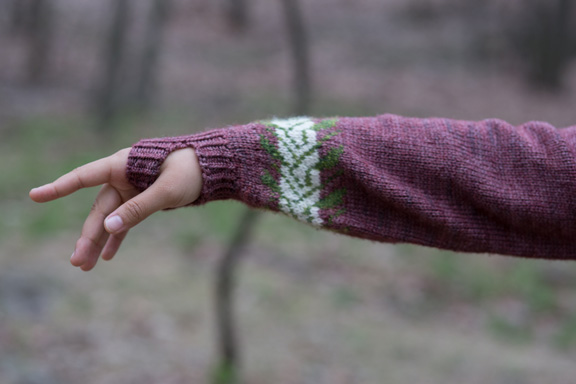
\includegraphics[width=0.9\linewidth]{hand.jpg}
\end{center}

\newpage

\section*{Finishing}

\subsection*{Folded Hem Collar}

Using MC and smaller needle, pick up and knit 
120 (126, 126, 126) (132, 132, 132) sts from the collar CO edge. Work 1x1 twisted ribbing for 2 inches, then fold collar to inside of the sweater so that sts on the needle line up with the CO edge. Bind off by sewing all live sts to the CO edge. \emph{See \textbf{Special Techniques} for detailed instructions on sewing down the collar.}

~\\
Use yarn ends at underarms to sew holes shut. Weave in all ends, but do not trim until after blocking. Gently block piece by soaking in cold water, pressing excess moisture out with a towel, and laying flat to dry. Enjoy your new sweater!

%%%%%%%%%%%%%%%%%%%%%%%%%%%%%%%%%%%%%%%%%%%%%%%%%%
% APPENDICES (IF ANY)

\section*{Special Techniques}
%% wrap & turn, working w&t's
\subsection*{Wrap \& Turn Short Rows}
\rowDir{w\&t on k side} start with yarn in back, slip 1 (as if to purl), bring yarn forward, slip back to L needle, bring yarn back, turn. \\
\rowDir{w\&t on p side} start with yarn in front, slip 1, bring yarn back, slip back to L needle, bring yarn forward, turn.

~\\
\emph{TIP: You may find it helpful to place a stitch marker after turning at the end of a w\&t.}


~\\
\rowDir{working a wrapped st on k side} insert needle into wrap as if to knit, insert needle into st as if to k, knit wrap and stitch together.

\rowDir{working a wrapped st on p side} insert needle back to front into the back half of the wrap, place on L needle like a st, p wrap and stitch together.


\vfill
\columnbreak

%% tubular bind off
\subsection*{Tubular Bind Off}
Work the following two set-up rounds:

\rowDir{Set Up Rnd 1} \repeat{slip 1 st purlwise with yarn in back, p1} to end of round. \\
\rowDir{Set Up Rnd 2} \repeat{k tbl, slip 1 st purlwise with yarn in front} to end of round.

~\\
Next, bring in an extra circular needle.

\rowDir{Next Rnd} slipping all sts purlwise, \repeat{slip 1 knit st to working needle, slip 1 knit st to extra needle} to end of round, until sts are divided in half between the two needles. Your working needle should be in front, and the extra needle in the back.

Cut yarn, leaving a tail 3 to 4 times the width/circumference of the work. Using a tapestry needle and this tail, use Kitchener stitch to graft the stitches on the front needle to those on the back needle.

~\\
\emph{Purl Soho} has an excellent \href{https://www.purlsoho.com/create/long-tail-tubular-bind-off/}{\underline{photo tutorial}} for this bind-off.

%% folded collar, sewing live sts to fabric
\subsection*{Sewing Down the Collar}
Cut working yarn, leaving a tail 3 to 4 times the circumference of the neckline. Thread through a tapestry needle.

~\\
\rowDir{Step 1} Insert tapestry needle purlwise into first st on L needle. Leave st on needle.

\rowDir{Step 2} Insert tapestry needle into corresponding bump in the CO edge.

\rowDir{Step 3} Insert tapestry needle knitwise into the same stitch in Step 1. Take stitch off the needle to bind off 1 st. 

~\\
Repeat Steps 1-3 until all stitches are bound off.

\begin{center}
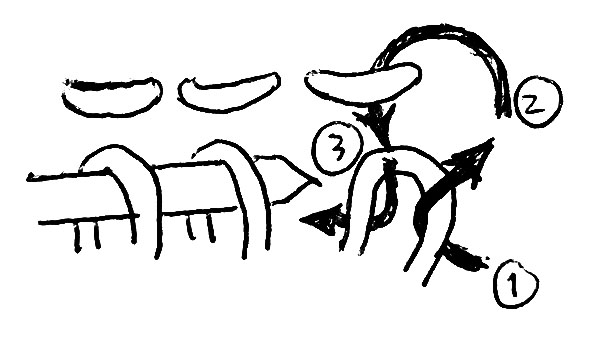
\includegraphics[height=1.5in]{sewing2.jpg}
\end{center}

\newpage
\section*{Modification Suggestions}

\emph{NOTE: Modifications may change yardage required to complete the sweater, mostly impacting MC.}

%% body and sleeve length
\subsection*{Adjusting Length}
If you are \vocab{modifying the body length}, work body until the piece measures 2"/5cm shorter than the desired length.

~\\
If you are \vocab{modifying the sleeve length}, begin the cuff colorwork when the piece measures 4"/10cm from the wrist. After the cuff colorwork, begin the ribbing when the piece measures 2 (2, 2.5, 2.5) (2.5, 3, 3)" or 5 (5, 6, 6) (6, 7, 7) cm shorter than the desired length.

%% body (bust/waist/belly) shaping
\subsection*{Large Bust Adjustment}

The sweater fit is based on a single measurement around the chest. However, a person with a large bust may wish to shape the sweater differently so that it sits properly on the neck and shoulders. One suggested modification is to adjust the round in which the yoke is divided for the body and sleeves so that the front is larger than the back.

\begin{enumerate}
\item Measure around the chest at the narrowest part, right underneath the armpits for the correct \textbf{chest measurement}. \blank

\item Next, measure around the chest at the fullest part of the bust for the \textbf{full bust measurement}. \blank

\item Take the difference between the two measurements. \blank

\item Multiply it by the stitch gauge to determine how many stitches to shift to the front of the work. \\
\blank" $\times$ 6 sts/1" $=$ \blank  \emph{or} \\ \blank cm $\times$ 6 sts $\div$ 10 cm $=$ \blank.

\item Refer to the round in \textbf{Separate for Body and Sleeves}. Note the number of knit stitches before the right sleeve. ``K \blank sts from marker \ldots" Subtract half of your result from Step 4. \blank

\item Referring to the same round, note the number of knit stitches for the front. ``\ldots k \blank sts for front \ldots" Add your result from Step 4. \blank
\end{enumerate}

If desired, work bust dart decreases while knitting the rest of the body.

\subsection*{Waist Shaping}
Waist shaping decreases can be worked along the sides of the sweater. When separating for the body and sleeves, mark the sides of the sweater by placing stitch markers at the middle of the underarm CO's. Every 2" or 5 cm in the body (spacing may depend on the desired shape), work the following decrease round.

\rowDir{Waist Decrease Round} k to 3 sts from side marker, k2tog, k1, sm, k1, ssk, k to 3 sts from other side marker, k2tog, k1, sm, k1, ssk, k to round marker.

\subsection*{A-line Shaping}
As the inverse of waist shaping, increases can be worked along the sides of the sweater to accommodate larger waists or hips.

%% swapping hand sizes
\subsection*{Changing Cuff Sizes}
Cuff Decrease Round 1 repeats a total of 8 (8, 8, 9) (9, 10, 10) times around. For a bigger cuff than what is written for your chosen size, omit the decreases in some of these repeats. For a smaller cuff than what is written for your chosen size, work Cuff Decrease Round 1 as written, then work Cuff Decrease Round 2.

\end{multicols}

\vfill
\begin{frnote} \ssmall
Pattern \copyright 2018 Shanel Wu. Photography by Vincent Villapando. All rights reserved. In purchasing this pattern, you agree to print and use this pattern only for personal use. Do not redistribute or sell paper or electronic copies of this pattern.
\end{frnote}

\end{document}